\documentclass[english]{cccconf}
%\documentclass[usemulticol,english]{cccconf}
% The preceding line is only needed to identify funding in the first footnote. If that is unneeded, please comment it out.
\usepackage{cite}
\usepackage{amsmath,amssymb,amsfonts}
\usepackage{algorithmic}
\usepackage{graphicx}
\usepackage{textcomp}
\usepackage{xcolor}
\usepackage{algorithm}
\def\BibTeX{{\rm B\kern-.05em{\sc i\kern-.025em b}\kern-.08em
    T\kern-.1667em\lower.7ex\hbox{E}\kern-.125emX}}
\begin{document}
\title{Clock Synchronization Scheme for Systems Using Integrated 5G and TSN Networks}
	

\author{San Zhang\aref{amss},
	Si Li\aref{amss,hit},
	Wu Wang\aref{hit}}

% Note: the first argument in the \affiliation command is optional.
% It defines a label for the affiliation which can be used in the \aref
% command. If there is only one affiliation for all authors, then the
% optional argument in the \affiliation command should be suppressed,
% and the \aref command should also be removed after each author in
% \author command, in this case the affiliation will not be numbered.

% Çë×¢Ò⣺\affiliationÃüÁîµÄµÚÒ»¸ö²ÎÊýÊÇ¿ÉÑ¡µÄ£¬Ëü¶¨ÒåÁËÓÃÓÚ\arefÃüÁîµÄ±êÇ©¡£
% Èç¹ûËùÓÐ×÷ÕßÖ»ÓÐÒ»¸öµ¥Î»£¬Ç벻ҪʹÓÃ\affiliationÃüÁîµÄ¿ÉÑ¡²ÎÊý£¬Í¬Ê±ÔÚÉÏÃæ
% µÄ\authorÃüÁîÖеÄÿλ×÷ÕßÐÕÃûºóÃæÒ²²»ÄÜʹÓÃ\arefÃüÁʾÀýÈçÏÂ
% \author{First Author, Second Author, Third Author}
% \affiliation{Chinese Academy of Sciences, Beijing 100190, P.~R.~China\email{ccc@amss.ac.cn}}
% ´Ëʱµ¥Î»Ç°²»»áÓÐÊý×Ö±àºÅ£¬×÷ÕßÐÕÃûºóÃæҲûÓбàºÅ

\affiliation[sjtu]{Department of Automation, Shanghai Jiao Tong University, Shanghai 200240, China}
\affiliation{*E-mail: wangwu@sjtu.edu.cn}  

\maketitle
\begin{abstract}
This article discusses the integration of IEEE 802.1 Time Sensitive Networking (TSN) and fifth-generation (5G) mobile technology in industrial communication networks. Clock synchronization is essential to achieve end-to-end deterministic connections between the two systems. However, current research only considers the simplest case of a single 5G bridge, whereas multiple bridges can increase cumulative synchronization error. To address this issue, the article proposes a clock synchronization scheme, a timestamp compensation scheme, and a carrier spacing optimization scheme for synchronization accuracy. The proposed algorithm is demonstrated through simulation. The paper provides valuable insights for multi-field manufacturing systems scenarios where multiple industrial Ethernet applications may work cooperatively through the 5G network in the time domain.
\end{abstract}

\keywords{IEEE 802.1 Time Sensitive Networking (TSN), fifth-generation (5G), clock synchronization, end-to-end deterministic connection}


\section{Introduction}
Industrial communication networks require high availability, reliability, and low latency. However, traditional industrial Ethernet systems are closed and incompatible with each other(shown in TABLE \uppercase\expandafter{\romannumeral1}). To improve real-time capabilities, the IEEE 802.1 Time Sensitive Network (TSN) standard is widely considered as a long-term substitute for proprietary technology in industrial control systems. Additionally, Industry 4.0 and Factory of Future (FoF) require wireless network access in Ethernet. Nevertheless, traditional wireless networks face problems of large transmission delay and short distance\cite{2013Recommendations}(shown in TABLE \uppercase\expandafter{\romannumeral2}). The fifth generation (5G) mobile/cellular technology, designed to support ultra-reliable low latency communication (URLLC), is expected to meet the strict requirements of industrial systems in the wireless field. Thus, the integrated operation of 5G and TSN systems is crucial to achieving end-to-end deterministic connection in industrial networks.
\begin{table}[!htb]
	\centering
	\caption{Current Main Ethernet Protocols}
	\label{tab1}
	\begin{tabular}{l|l|l}
			\hline
\textbf{Protocol}& \textbf{Organization}& \textbf{Manufacturer} \\
\hline
EtherNet/IP
& ODVA
& Rockwell \\
\hline
PROFINET
& PROFIBUS
& Siemens \\
\hline
EtherCAT
& EtherCAT Association
& Bev \\
\hline
POWERLINK
& EPSG
& ABB \\
\hline
CC-LINK
& CC-Link Association
& Mitsubishi \\
\hline
	\end{tabular}
\end{table}
\begin{table}[!htb]
	\centering
	\caption{Current Main Wireless Protocols}
	\label{tab1}
	\begin{tabular}{l|l|l}
\hline
\textbf{Protocol}& \textbf{Delay}& \textbf{Transmission Distance} \\
\hline
LTE
& 6ms
& 400-1000m \\
\hline
WIFI
& 6ms
& 100-200m \\
\hline
Zigbee
& 1-3ms
& 10-100m \\
\hline		
	\end{tabular}
\end{table}
Clock synchronization is the basis and key of 5G+TSN integration. The 3GPP protocol proposes a bridge architecture synchronization mode based on TSN802.1AS for clock synchronization, but specific synchronization rules and algorithm details are not specified\cite{888888}. Previous research analyzed the impact of various errors that may exist at the junction of the bridge and TSN nodes in the synchronization architecture on the synchronization algorithm\cite{9527833}. Research\cite{9211936} optimized the synchronization packets inside the 5G bridge, reducing communication overhead. Another study has introduced a clock domain compensation technology to estimate the residence time of 5G timing messages\cite{9674640}, and another research work has investigated how synchronization and syntonization errors affect the achievable end-to-end time synchronization accuracy in integrated 5G and TSN networks However, current research only considers the simplest case of a single 5G bridge\cite{9557468}. In future intelligent factories integrated with industrial and 5G networks, multiple industrial Ethernet application scenarios may work cooperatively through the 5G network in the time domain\cite{8402373}(Fig.1). When multiple bridges are present in a system, the cumulative synchronization error can increase. Therefore, this paper proposes the following contributions to address these issues:
\begin{itemize}
	\item we propose a clock synchronization scheme for multi-field manufacturing systems scenarios.
	\item we propose a timestamp compensation scheme for multi-hop synchronization errors in multi-field manufacturing systems scenarios.
	\item we propose a carrier spacing optimization scheme for synchronization accuracy in 5G+TSN clock synchronization.
\end{itemize}
\begin{figure}[htbp]
	\centering
	\setcounter{figure}{0}
	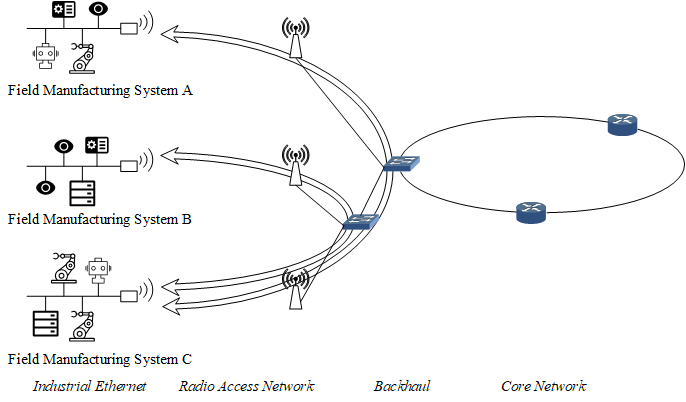
\includegraphics[width=3in]{fig11.png}
	\caption{Multi-field Manufacturing Systems Scenarios}
	% \label{fig_sim}
\end{figure}

The paper is structured as follows: In Chapter \uppercase\expandafter{\romannumeral2}, we analyze the clock model and error model. In Chapter \uppercase\expandafter{\romannumeral3}, we propose a hybrid synchronous architecture that uses 5G+TSN as the core network to address the synchronization needs of multi-field manufacturing systems scenarios. In Chapter \uppercase\expandafter{\romannumeral4}, we optimize the cumulative error in the synchronization process by carrier spacing optimization and timestamp compensation. In Chapter \uppercase\expandafter{\romannumeral5}, we demonstrate the algorithm's effect through simulation.

\section{Model}

\subsection{Clock Model}
The complexity of the industrial site can significantly affect the crystal oscillator of the device clock, leading to deviations in the initial clock state and rate of change, resulting in clock errors. Specifically, the clock of a node can be expressed as:
\begin{equation}
	C_i(t) = (\alpha _i+\sigma_i)t + \beta _i +\delta_i
\end{equation}
where $\alpha_i$ and $\beta_i$ are the estimated time-varying clock skew and constant clock offset to the reference clock, and $\sigma_i$ and $\delta_i$ are the errors in the estimation of the frequency and time differences. Ideally, $\alpha_i = 1$ and $\beta_i = 0$. The change in slope arises from the drift of the internal crystal oscillator of the clock, while the difference in the initial state results from errors during network initialization. The crystal frequency of the clock is affected by various factors, such as temperature, voltage, and aging degree, among others.

In the 5G-TSN bridge structure (as shown in Fig.2), 5G and TSN networks operate in different time domains. Therefore, for the current bridge structure combined with 5G and TSN, the clock model of the TSN time domain can be expressed as:
\begin{equation}
	C_{TSN}(t) = (\alpha_{TSN}+\sigma_{TSN})t + \beta _{TSN} +\delta_{TSN}
\end{equation}
 correspondingly, the clock model of the 5G part can be expressed as:
 \begin{equation}
 	C_{5G}(t) = (\alpha_{5G}+\sigma_{5G})t + \beta _{5G} +\delta_{5G}
 \end{equation}
in these equations, $\alpha_{TSN}$ and $\sigma_{TSN}$ represent the frequency synchronization correction estimate and error on the wired side, respectively. Similarly, $\alpha_{5G}$ and $\sigma_{5G}$ represent the frequency synchronization correction estimate and error on the wireless side. $\beta_{TSN}$ and $\delta_{TSN}$ represent the time bias synchronization correction estimate and error on the wired side, while $\beta_{5G}$ and $\delta_{5G}$ represent the estimated value and error of the time-bias synchronization correction on the wireless side. 

In the given equations, it is assumed that the synchronization errors $\sigma_{TSN}$ and $\delta_{TSN}$ are much smaller than those of the 5G network, $\sigma_{5G}$ and $\delta_{5G}$. Typically, the synchronization accuracy of the 5G network is at the microsecond level, while that of the TSN network is at the nanosecond level. Hence, when timestamps pass through the bridge, there are bound to be timestamp errors. These errors are usually acceptable when only one bridge is present, but in scenarios where there are multiple bridges in the network, the errors accumulate and significantly impact clock synchronization. These timestamp errors impact synchronization accuracy by affecting the measurement of delay during clock synchronization. Therefore, in order to address these errors, we need to model and analyze the delay.
\begin{figure}[htbp]
	\centering
	\setcounter{figure}{1}
	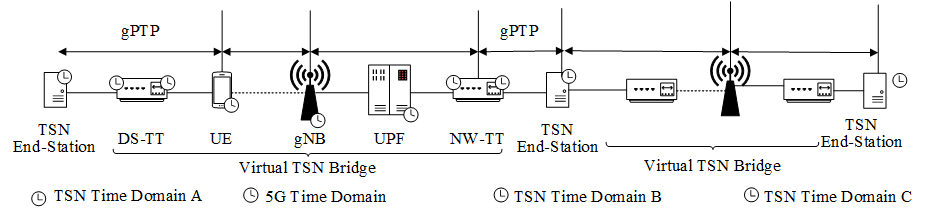
\includegraphics[width=3.5in]{fig12.png}
	\caption{5G-TSN Bridge}
	% \label{fig_sim}
\end{figure}
\subsection{Delay Model}
In the process of synchronization, in addition to the accuracy of the clock, the delay between nodes is an important factor that affects synchronization accuracy. In the network bridge structure, the 5G network bridge is composed of all 5G wireless nodes that relay the signal. Therefore, the transmission delay between the internal nodes of the 5G network determines the transmission delay of the network bridge, thereby affecting the clock synchronization accuracy of the TSN devices at both ends. Typically, the delay can be expressed as:
\begin{equation}
	Delay=D_d+D_r
\end{equation}
where $D_d$ is the deterministic delay, mostly composed of transmission delay that can be measured or eliminated. On the other hand, $D_r$ is the random delay, mostly composed of propagation delay jitter and cumulative error. While propagation delay jitter can be periodically measured to reduce its effect on synchronization accuracy\cite{9064350}, accumulated errors may have a significant impact on clock synchronization accuracy in large-scale networks. To analyze the specific effects of accumulated error, it is necessary to model the queuing delay.
\begin{figure}[htbp]
	\centering
	\setcounter{figure}{2}
	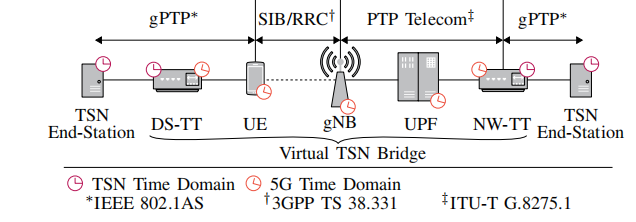
\includegraphics[width=3.5in]{fig3.png}
	\caption{the Internal Synchronization Mode of 5G }
	% \label{fig_sim}
\end{figure}
The internal synchronization mode of the 5G network is illustrated in Fig.3, where 5G wireless nodes synchronize by receiving Sync messages from the base station. When multiple nodes synchronize with the same base station simultaneously, queuing delay occurs. To calculate the expected value of the queuing delay, the queue generated by the non-clock-synchronous traffic arriving in batches at the switch is computed first, and the expected value of the series is obtained by calculating the generating function of the series. Then, the queue delay of the clock-synchronous flow in the presence of background traffic is analyzed to obtain the expected length of the queue. The calculation of background traffic adopts the non-preemptive consideration, which is more in line with the actual situation. Both the non-clock synchronous traffic queue and clock-synchronous traffic queue are modeled, and queuing theory is used to model and solve the Markov chain. The steady-state equation listed according to the Markov chain is:

\begin{equation*}
	p_i\left( \lambda +i\cdot \mu \right) =\sum_{j=0}^i{p_j\cdot \lambda \cdot a_{i-j}+p_{i+1}\left( i+1 \right) \cdot \mu\,\, 0\leqslant i<m}
\end{equation*}
\begin{equation}
	p_i\left( \lambda +m\cdot \mu \right) =\sum_{j=0}^i{p_j\cdot \lambda \cdot a_{i-j}+p_{i+1}m\cdot \mu}\,\, m\leqslant i
\end{equation}
where $p_i$ is the probability of there being $i$ packets in the queue, $m$ is the maximum queue value, $\lambda$ is the total packet arrival rate, $\mu$ is the packet processing rate, and $a$ is the distribution of the number of packets arriving.And $c=\mu/\lambda $.We assume that when $k$ packets arrive at the base station, there are $v$ non-clock synchronous packets in the system. There can be three cases:
\begin{itemize}
	\item Case 1: $v<m$,$k<m-v$, QueueLength = 0.
	\item Case 2: $v<m$,$k>m-v$, QueueLength = $k+v-m$.
	\item Case 3: $v>m$, QueueLength = $k$.
\end{itemize}

Based on these three cases, the expected value of queuing delay can be obtained by solving the Markov chain and summing with the full probability formula.
\begin{equation*}
	L_q=P_0\cdot \sum_{i=0}^m{\left(k-m+i\right)\cdot \frac{\left(\lambda/\mu\right)^i}{i!}+P_0\cdot \frac{k-m}{m!}\cdot \frac{\rho^m}{v!\left(1-\rho^m\right)}}
\end{equation*}
\begin{equation}
	\rho=\frac{\lambda}{\mu}
\end{equation}

According to the 5G protocol standard 3GPP TS 22.104 for large-scale application scenarios (3GPP, 2020), the upper limit of synchronization nodes in a single time domain is 100 when the service area is between 10 and 20 $km^2$\cite{888889}. By substituting these conditions into the queuing delay model, we can ensure that the queuing delay is less than 250 ns. Given the required synchronization accuracy of $1\mu s$, we can assume that the random queuing delay has a negligible influence on the synchronization accuracy, and that only the fixed delay impacts synchronization accuracy. Therefore, our timestamp compensation for multi-field manufacturing systems scenarios can focus solely on the effect of fixed delay on clock synchronization under these conditions.

\section{Synchronization Architecture}
\subsection{Network Structure}
To address multi-field manufacturing system scenarios, we have designed a synchronization architecture for heterogeneous networks. This architecture involves dividing the industrial Ethernet network into different wired islands based on the clock model's different time-domain models. The 5G network acts as a bridge between these wired islands. In 3GPP, two main clock models are considered for time synchronization in integrated 5G and TSN systems, both of which comply with the IEEE 802.1AS standard. These models include the boundary clock and the transparent clock\cite{9615318}.

In the boundary clock solution, the 5G Radio Access Network (RAN) has direct access to the TSN master clock, providing timing information to user equipment (UE) through its own signaling and procedures. UE synchronizes TSN devices based on periodic information. In contrast, the transparent clock solution achieves time synchronization by exchanging PTP messages, where any intermediate 5G or TSN entity between the TSN main console and the TSN device will update the PTP message to update the time spent in the entity.

Therefore, 5G networks serve as transparent clocks, while wired networks serve as boundary nodes. The 5G RAN has direct access to the TSN Master Time, either through a direct connection to the TSN master clock or through an underlying transport network that supports PTP, which can reduce the transmission overhead of TSN timestamps in 5G networks.

To meet the requirements of assumptions and communication protocols, the number of wireless nodes in each network bridge should not exceed 100. When the number of nodes exceeds this number, a new boundary node will be established to split the network bridge. Figure 3 shows the overall architecture diagram.
\begin{figure}[htbp]
	\centering
	\setcounter{figure}{3}
	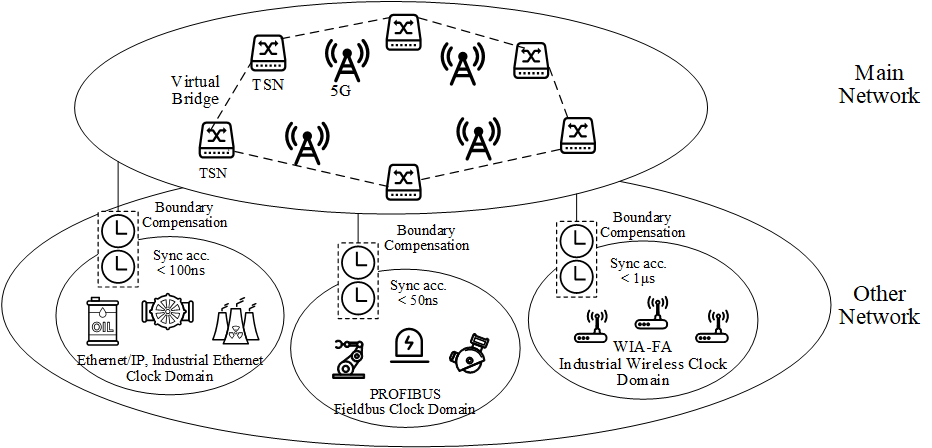
\includegraphics[width=3.5in]{fig17.png}
	\caption{Schematic of slot allocation in the TAS model}
	% \label{fig_sim}
\end{figure}
\subsection{Synchronization Mechanism}
To synchronize the wired part, we adopt the GPTP synchronization scheme, while broadcast synchronization completes the synchronization of the wireless part. The accuracy of the synchronization within the 5G bridge affects the precision of the time calculation when the timestamp passes through the transparent clock. To synchronize the clock of a multi-hop large-scale wireless network node inside the 5G-TSN bridge, we first need to determine the hierarchy of each node, which forms the basis for locating each wireless node.

The root node initiates the synchronization message with a count of $k=0$, and the receiving node sets the count to $k+1$ and sends the broadcast synchronization message containing $k+1$ to the next level. To minimize energy consumption and reduce computational complexity while maintaining synchronization accuracy, we adopt the mechanism of inverse synchronization for the asymmetric network clock synchronization characteristics of the TSN+5G network\cite{8935413}. Timestamp conversion involves floating-point division, which needs to be performed at the TSN end since it has more computational resources.

Specifically, the 5G nodes periodically launch synchronization request messages to the TSN switches of the edge nodes at both ends. The slave clock receives the reference timestamp $G$ from the master clock through several intermediate ones and records the local time $L$, which are then sent to the TSN nodes. The TSN node performs a linear regression process to estimate the frequency difference and clock deviation after exchanging several sets of timestamps. The intermediate forwarding node is treated as a transparent clock.

Finally, the correction time of each wireless node can be expressed as follows:
Please find below the proofread text:

The correction time of each wireless node can be expressed as:
\begin{equation}
	\widehat{L}=L\left(1+\frac{\widehat{\alpha}}{f_0}\right)-\widehat{\beta}+\left[\frac{G_0-L_0}{T_c}\right] T_c
\end{equation}
where $\widehat{\alpha}$ represents the estimation of frequency difference, and $\widehat{\beta}$ is the estimation of clock deviation.The term $[\frac{G_0-L_0}{T_c}] T_c$ represents the transmission delay from the 5G network node to the TSN node. $T_c$ represents the time slot of the 5G network and is the upper limit of accuracy that can be achieved by estimating the transmission delay during the 5G-TSN clock synchronization. This forms the basis for the subsequent synchronization accuracy optimization scheme.
\section{Synchronization Error}

\subsection{Optimization}
According to Equation (7), the upper limit of error for estimating transmission delay during 5G-TSN synchronization in 5G networks is known to be $T_c/2$. As shown in Figure 5, the frame structure of 5G networks consists of a wireless frame and a subframe of the same length, which are 10ms and 1ms, respectively. Each time slot in 5G contains 14 OFDM symbols, with 4 OFDM symbols occupied by SSBS (clock synchronization messages). The duration and period of SSBS vary with different subcarrier intervals, and the interval of 5G subcarriers can be adjusted. By utilizing the distributable property of the subcarrier interval in 5G networks, the number of subcarriers and the symbol length of OFDM can be reduced by increasing the subcarrier interval, thereby reducing delay and cumulative error. From these protocols we can obtain Equation 8:
\begin{equation}
	\begin{split}
		&T_{c}=\frac{15kHz}{\triangle F}\\
		&\triangle F=2^\mu\cdot15kHz \\
	\end{split}	
\end{equation}
where $\triangle F$ is the sub-carrier spacing (SCS), $\mu=\{0,1,2,3,4,5\}$. It shows that when the active carrier bandwidth $f_c$ is fixed, increasing the sub-carrier spacing $\triangle F$ decreases clock synchronization errors $\varepsilon$.

However, increasing the carrier spacing can also cause the following problems:
\begin{itemize}
	\item reduced spectral efficiency: the larger the carrier interval, the smaller the amount of data that can be transmitted on each carrier, and the lower the spectral efficiency.
	
	\item reduced anti-interference capability: the larger the carrier spacing, the larger the channel width, and the larger the BER when encountering interference sources.
	
	\item increased power consumption: if the BER(Bit Error Rate) is to be guaranteed low, the signal power needs to be enhanced, which will lead to increased power consumption.
	
	\item waste of resources: a large carrier spacing may cause some spectrum resources to be wasted.
\end{itemize}
Choosing an appropriate carrier spacing is crucial for achieving high-precision 5G+TSN synchronization. This problem can be reduced to a trade-off between synchronization accuracy and bandwidth utilization, which can be expressed as:
\begin{equation}
	\eta=f_c\cdot \frac{B}{12\cdot N_{RB}\cdot \triangle F}
\end{equation}
where $N_{RB}$ is the number of RBs, and $B$ is the network's bandwidth. To find the optimal carrier spacing, an optimization problem can be constructed as follows:
\begin{equation}
	\begin{split}
		&\min_{\triangle F} \,\, \omega_1 \cdot T_c+\omega_2 \cdot \frac{1}{\eta} \\
		&s.t.\quad  \left\{\begin{array}{lc}
			T_{cmin}\leq T_c \leq T_{cmax}\\
			B_{min}\leq B \leq B_{max}\\
			N_{RB}\leq 273\\
		\end{array}\right.
	\end{split}
\end{equation}
where $\omega_1$ and $\omega_2$ represent the weights of synchronization accuracy and bandwidth utilization, respectively. Users can assign their weights according to their needs. This method minimizes synchronization errors without significantly impacting the original communication quality of the 5G network.
\begin{figure}[htbp]
	\centering
	\setcounter{figure}{4}
	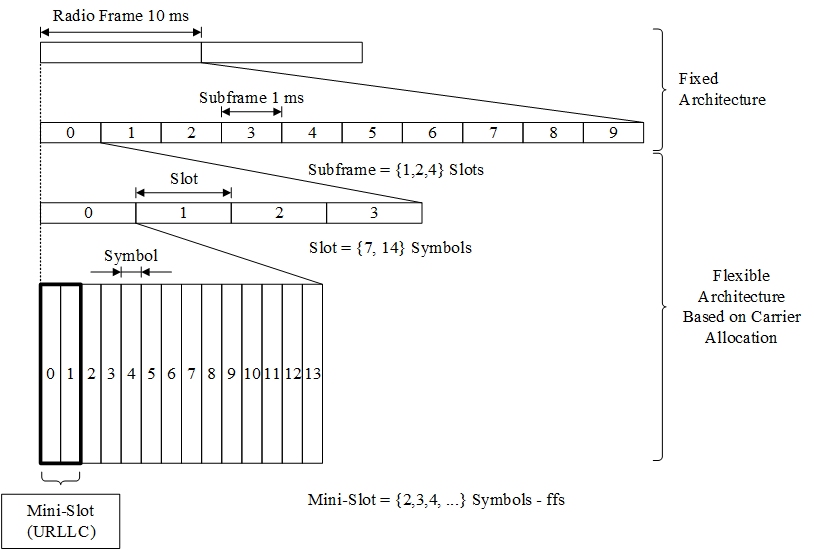
\includegraphics[width=3in]{fig14.png}
	\caption{5G Carrier Structure}
	% \label{fig_sim}
\end{figure}
\subsection{Compensation}
When multiple bridges are connected to each other in the network, as shown in Fig.1, the cumulative error will be further amplified, and the timestamp needs to be compensated and corrected. At each point where the Time-Sensitive Networking (TSN) network intersects with the 5G network, the synchronization process can be represented as in Fig.5. The TSN time domain at both ends can be abstracted as master-slave nodes. According to equations 2 and 3, the local time of the wired and wireless sides can be expressed as:
\begin{eqnarray}
	\begin{aligned}
		&t_{(\text {wired})}=\left(\alpha_{TSN}+\sigma_{TSN}\right) t+\beta_{TSN}+\delta_{TSN}\\
		&t_{(\text {wireless })}=\left(\alpha_{5G}+\sigma_{5G}\right) t+\beta_{5G}+\delta_{5G}\\
	\end{aligned}
\end{eqnarray}
Due to differences in the accuracy of time bias and frequency estimation on both sides, clock synchronization between wired and wireless timestamp exchanges can cause boundary synchronization errors.When the left wired master clock sends a sync message containing a timestamp of time $t_1$, the corresponding reference time should be $t_1^{ref}$. When this message arrives on the wireless side, the node will receive and record the timestamp $t_2$. The timestamp values can be expressed as follows:
\begin{equation}
	\begin{split}
		&t_{2}=(t_1^{ref}+delay)(\alpha_{5G}+\sigma_{5G})+\beta_{5G}+\delta_{5G} \\
		&t_1^{ref}=\frac{t_{1}-\beta_{TSN}-\delta_{TSN}}{\alpha_{TSN}+\sigma_{TSN}}
	\end{split}
\end{equation}
similarly, on the wireless network side, the node records the timestamp $t_3$ upon receiving the $Sync$ message and sends the  $Delay\_Req$ message. Subsequently, the wired network node records the timestamp $t_4$ after receiving  $Delay\_Req$. The values of the timestamps can be expressed as:
\begin{equation}
	\begin{split}
		&t_{4}=(t_3^{ref}+delay)(\alpha_{TSN}+\sigma_{TSN})+\beta_{TSN}+\delta_{TSN} \\
		&t_3^{ref}=\frac{t_{3}-\beta_{5G}-\delta_{5G}}{\alpha_{5G}+\sigma_{5G}}
	\end{split}
\end{equation}
thus the transmission delay between the two network nodes can be expressed as:
\begin{equation}
	\begin{split}
		&2  delay =t_{2}-t_{1}+t_{4}-t_{3} \\
		&=m\left(t_{2}-t_{1}+t_{4}-t_{3}\right)-(m-1 / m)\left(\beta_{TSN}+\delta_{TSN}\right)\\
		&\quad+(m-1 / m)\left(\beta_{5G}+\delta_{5G}\right)\\
		& \approx m\left(t_{2}-t_{1}+t_{4}-t_{3}\right)-(m-1 / m)\left(\beta_{5G}+\delta_{5G}\right)\\
		&m=\frac{\alpha_{5G}+\sigma_{5G}}{\alpha_{TSN}+\sigma_{TSN}}		
	\end{split}
\end{equation}
in equation 14, the synchronization error of the wired part is much smaller than that of the wireless part and is therefore neglected. It is important to note that the calculation of the timestamp and clock parameters should be performed on the side of the wired network (i.e., the TSN node), and then the result should be sent to the 5G network node via the $Delay\_Resp$ message. The synchronization algorithm involves floating-point division, and because TSN network nodes have higher accuracy in floating-point calculation, these calculations should be performed by the head (TSN) part. This can effectively improve synchronization accuracy and reduce the computational complexity of 5G nodes.

\begin{figure}[htbp]
	\centering
	\setcounter{figure}{5}
	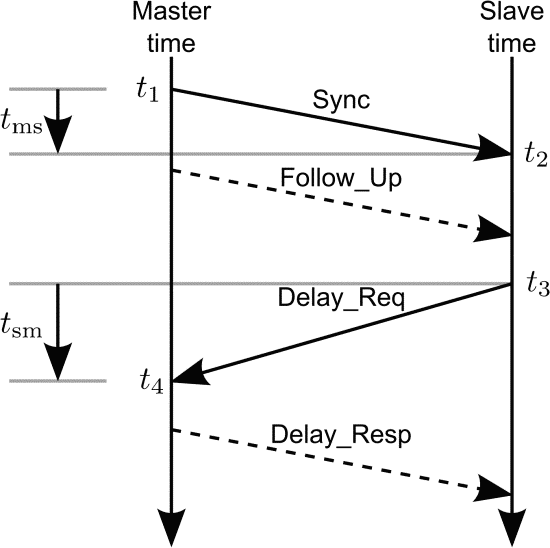
\includegraphics[width=2in]{fig10.png}
	\caption{Synchronization process}
	% \label{fig_sim}
\end{figure}
\section{Simulation Results}
Based on the proposed synchronization architecture and model in Chapters 2 and 3, we conducted numerical simulations to evaluate the optimization and compensation schemes' performance. Initially, we examined the synchronization accuracy at various subcarrier spacing (SCS) values. Following the numerology setting of 5G NR system \cite{access2015requirements}, the maximum SCS is 480 kHz, and the Fourier transform (FFT) size is 4096, resulting in a time unit of 0.509 ns. We assumed the 5G internal UE clock drift compared to the gNB clock, $\frac{\alpha_{5G}}{\alpha_{TSN}}$, to be 10 ppm (10 ns per millisecond). Table 3 shows the simulation results.

Based on our proposed synchronization architecture and model in Chapter 2 and 3, numerical simulations were performed to evaluate the performance of the optimization and compensation schemes. First, we tested the values of synchronization accuracy at different SCSs. According to the numerology setting of 5G NR system\cite{access2015requirements}, the maximum SCS $\triangle F_{max}$ is 480 kHz and the FFT(Fourier transform) size is 4096, thus conducting to a time unit covering 0.509 ns. We set the drift of the 5G internal UE clock compared to the gNB clock, $\frac{\alpha_{5G}}{\alpha_{TSN}}$, to 10 ppm (10 ns per millisecond).The results of the simulation are shown in Table 3.
\begin{table}[!htb]
	\centering
	\caption{Carrier Spacing and Synchronization Errors}
	\label{tab1}
	\begin{tabular}{l|l|l}
		\hline
		 & \textbf{mean error(ns)}& \textbf{max error(ns)} \\
		\hline
		15kHz 
		& 896
		& 2525 \\
		\hline
		30kHz
		& 425
		& 1295 \\
		\hline
		60kHz
		& 295
		& 899 \\
		\hline
		120kHz
		& 135
		& 578 \\
		\hline
		240kHz
		& 120
		& 512 \\
		\hline
			480kHz
		& 112
		& 508 \\
		\hline
	\end{tabular}
\end{table}

It can be learned that when the SCS increases, the synchronization error decreases, but when the SCS reaches 120 kHz, the error decreases slowly, and when it reaches 240 kHz, the error size tends to a constant value.
Then the weights of synchronization accuracy and bandwidth utilization($\omega_1,\omega_2$) are set to (0.5,0.5). By solving the optimization problem in Chapter 4, we can get the optimal performance when the carrier bandwidth is 120kHz, at which time the total available bandwidth length is 393.12MHz, the utilization rate hit 98\%, reaching the highest utilization rate of the 5G network, while the available bandwidth utilization rate is 83. 38\%, meeting most of the transmission need.
After determining the most suitable carrier interval, we simulated the timestamp compensation in Chapter 4.
We model each mobile robot as a TSN endstation, connected to a 5G UE via a variable number of TSN Bridges (here: transparent clocks). Every device, both TSN and 5G, is based on the omnet node class. The Node classes are described as follows: 
\begin{itemize}
	\item The TSN nodes in the network are linked through the Carrier Sense Multiple Access (CSMA) channel model, which supports layer 2 communication and is a suitable approximation of ethernet for the purpose of the network. A separate class defines the gPTP (Generalized Precision Time Protocol) procedures that are installed on each node. The nodes are differentiated into ordinary and transparent clocks, determining how they interact with different gPTP messages. Each TSN node starts the peer delay messaging process with its neighbors, while only the ordinary clock, acting as the master clock, initiates the synchronization messaging process.
	\item The TSN nodes in the network are connected via a Carrier Sense Multiple Access (CSMA) channel model, which supports Layer 2 communications and meets the specification requirements of 802.1AS. A separate class defines the gPTP (Generic Precision Time Protocol) program installed on each node. The node types are divided into boundary clocks and common clocks, which determine their different modes of behavior. The common node performs the transmission delay measurement procedure by receiving synchronization information from the master clock, while the boundary node performs the transmission delay measurement procedure as the master clock after receiving the synchronization requirements from the 5G node.
\end{itemize}
The nodes in the network are arranged according to the structure of a binary tree, in the multi-bridge scenario of clock synchronization, the errors in multiple bridges will have probability of canceling each other out, and the error size will fluctuate within a range, we conducted 100 simulations for each different number of bridges in the size of the network, and obtained the Fig.7.
\begin{figure}[htbp]
	\centering
	\setcounter{figure}{6}
	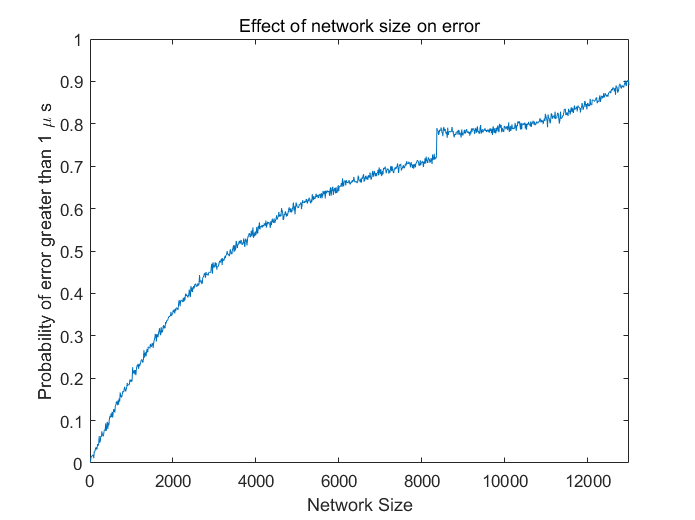
\includegraphics[width=2in]{fig18.png}
	\caption{Error probability}
	% \label{fig_sim}
\end{figure}

The graph represents the relationship between the probability of error greater than 1 $\mu s$ and the accuracy requirement and the network size, which is represented by the numbers of 5G-TSN bridges.It can be seen from the figure that when the network size keeps increasing and the number of 5G-TSN bridges keeps increasing, the probability that the synchronization accuracy exceeds the minimum requirement of the accuracy requirement becomes higher and higher, and when the number of bridges reaches 13000, the synchronization error will have more than 90\% probability of being above 1 $\mu s$. Therefore, the algorithm in Chapter 4 is used to compensate for the timestamp, and the results after compensation are compared as follows.
\begin{figure}[htbp]
	\centering
	\setcounter{figure}{6}
	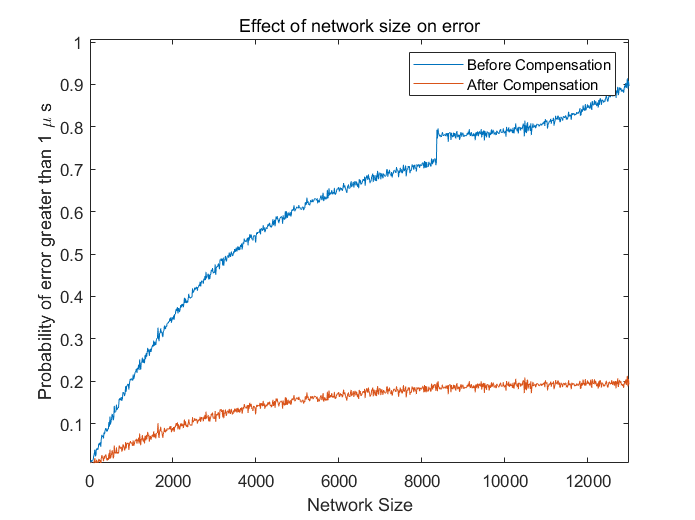
\includegraphics[width=2in]{fig20.png}
	\caption{Comparison of error probability }
	% \label{fig_sim}
\end{figure}
\begin{figure}[htbp]
	\centering
	\setcounter{figure}{7}
	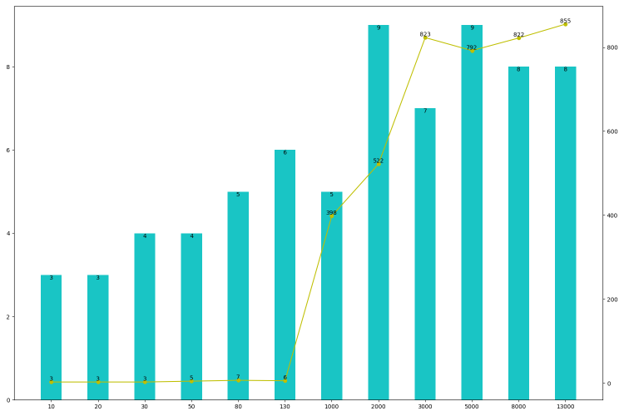
\includegraphics[width=2in]{fig19.png}
	\caption{Average error comparison}
	% \label{fig_sim}
\end{figure}

\bibliography{cx.bib}
\bibliographystyle{IEEEtran}
\end{document}
